\section{Unified Modeling Language (UML)}

\hspace{1cm} The Unified Modeling Language (UML) is a graphical language for 
visualizing, specifying, constructing, and documenting software-intensive systems. 
This language is maintained by the Object Management Group (OMG) \cite{UML}.

UML serves as a standardized modeling language for visualizing and documenting 
software-intensive systems \cite{UML}. It incorporates various object-oriented 
and component-based methods to represent software architectures and designs. 
Software development projects face inherent complexity challenges when systems 
increase in size, functionality, and distribution across networks. UML addresses 
these challenges by offering structured graphical representations that abstract 
complex systems into comprehensible models, capturing essential structural and 
behavioral elements required for effective design and implementation processes. 
The notation system provides developers with a common vocabulary for communicating 
system architecture and behavior among stakeholders \cite{UML_Reference_Manual}.
% UML is one of the most widely used modeling languages for describing real-world 
% application domains. It works with various object and component methods to represent 
% software systems. As software systems grow in size, complexity, and distribution, 
% building and maintaining them becomes more challenging. UML helps reduce this 
% complexity by providing a high level of abstraction that captures essential 
% information needed for designing and developing software systems.

UML includes multiple diagram types, each focusing on different aspects of a design. 
These diagrams fall into two main categories: (1) structural diagrams that represent 
the static aspects of a system, and (2) behavioral diagrams that describe the dynamic 
aspects. These structural and behavioral categories collectively contain fourteen 
different diagram types, as specified in the UML Reference Manual \cite{UML_Reference_Manual}.

For this thesis, two related structural diagrams are particularly relevant and will be presented in the following subsections: class diagrams, which define the abstract structure of a system, and object diagrams, which provide concrete instances of that structure.


\subsection{Class Diagram}
\hspace{1cm} Class diagrams are the foundation of structural modeling in UML and the most widely 
used diagram type in object-oriented systems. They illustrate the static structure 
of a system by depicting classes, their attributes, operations, and the relationships 
between classes. These concepts can be observed in Figure 
\ref{fig:class_diagram_bank_account_model} adapted from \cite{TPV}, 
which shows a class diagram of a simple bank account system.

\begin{figure}
    \begin{center}
        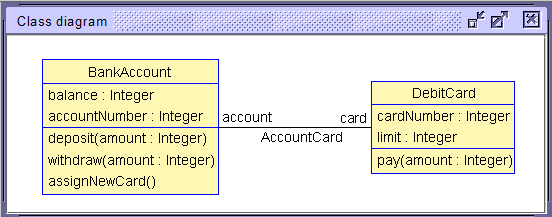
\includegraphics[width=0.8\textwidth]{figures/c1/BankAccount/BankAccount_ClassDiagram.png}
        \caption{Class diagram of the Bank Account Model adapted from \cite{TPV}.}
        \label{fig:class_diagram_bank_account_model}
    \end{center}
\end{figure}

In this diagram, we see two classes, \texttt{BankAccount} and \texttt{DebitCard}, 
which represent sets of objects that share common characteristics. Each class 
contains attributes that describe the data values their objects may contain. 
The \texttt{BankAccount} class has attributes such as:
\begin{itemize}
    \item \texttt{accountNumber}: a unique identifier for the bank account
    \item \texttt{balance}: the current balance of the bank account
\end{itemize}
Similarly, the \texttt{DebitCard} class has attributes:
\begin{itemize}
    \item \texttt{cardNumber}: a unique identifier for the debit card
    \item \texttt{limit}: the maximum amount that can be withdrawn using the debit card
\end{itemize}

Classes also include operations that specify the behaviors objects can perform. 
In our example, the \texttt{BankAccount} class defines three operations:
\begin{itemize}
    \item \texttt{deposit(amount)}: adds the specified amount to the account balance
    \item \texttt{withdraw(amount)}: deducts the specified amount from the balance
    \item \texttt{assignNewCard()}: creates and assigns a new debit card to the bank account
\end{itemize}

These operations represent the functional capabilities of \texttt{BankAccount} objects, 
defining how they can interact with other objects and how their state can change over 
time. While attributes describe what an object knows, operations describe what an 
object can do.

Relationships between these classes are represented by the \texttt{AccountCard} 
association, which connects \texttt{BankAccount} and \texttt{DebitCard}. 
Multiplicity indicators on this association would show how many objects of one class 
can be linked to objects of another class. In addition to simple associations like 
this one, class diagrams can include more specialized relationship types: aggregation 
and composition (both representing whole-part relationships with different levels of 
dependency), and generalization (inheritance relationships where specialized classes 
inherit properties from a general class).

Class diagrams represent the static structure of a system at a particular point in 
time, providing the vocabulary and structural framework that other diagrams and 
behavioral specifications build upon.


\subsection{Object Diagram}
\hspace{1cm} Object diagrams are structural diagrams that represent real-world entities or 
modeled system elements as concrete instances of classes. While class diagrams 
show abstract structures, object diagrams provide snapshots of a system at specific 
points in time, showing actual objects with specific attribute values and the links 
connecting them.

\begin{figure}
    \begin{center}
        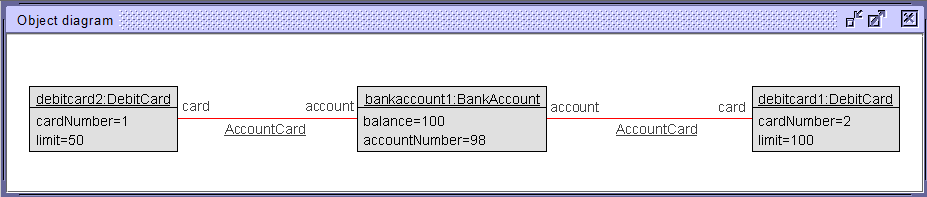
\includegraphics[width=0.8\textwidth]{figures/c1/BankAccount/BA_ObjectDiagram.png}
        \caption{Object diagram of the Bank Account Model.}
        \label{fig:object_diagram_bank_account_model}
    \end{center}
\end{figure}

Figure \ref{fig:object_diagram_bank_account_model} shows an example object diagram for the banking system previously described in the class diagram (Figure \ref{fig:class_diagram_bank_account_model}).
The links between objects in the diagram represent instances of the associations defined in the class diagram. Here, the \texttt{AccountCard} links connect the \texttt{bankaccount1} object to both debit card objects, showing that this particular bank account has two associated debit cards with different withdrawal limits.

Object diagrams provide concrete examples that help verify that a system model behaves as expected. They are valuable for validating class structures, illustrating complex relationships, and demonstrating specific scenarios during system design. While object diagrams excel at representing static information about system states, they do not capture the dynamic interactions that cause state changes. This characteristic defines both the strength and scope of object diagrams within UML modeling - they offer precise snapshots of system state at a particular moment in time, complementing the abstract structural representations provided by class diagrams.

